\documentclass[aspectratio=169]{beamer}
\usetheme{Madrid}
\usefonttheme{structurebold}
\usefonttheme[onlymath]{serif}

\definecolor{BKTemplate}{rgb}{0.11765, 0.30588, 0.47451}
\usecolortheme[named=BKTemplate]{structure}
\setbeamercolor{title}{fg=BKTemplate,bg=}
\setbeamertemplate{caption}[numbered]

% Engine-adaptive font configuration
\usepackage{iftex}
\ifLuaTeX
  \usepackage{fontspec}
  \setmainfont{Noto Sans}
  \setsansfont{Noto Sans}
  \setmonofont{Noto Sans Mono}
\else\ifXeTeX
  \usepackage{fontspec}
  \setmainfont{Noto Sans}
  \setsansfont{Noto Sans}
  \setmonofont{Noto Sans Mono}
\else
  \usepackage[utf8]{inputenc}
  \usepackage[T5,T1]{fontenc}
\fi\fi

\usepackage[english,vietnamese]{babel}
\usepackage{url}
\usepackage{booktabs}
\usepackage{array}
\usepackage{amsfonts}
\usepackage{amsmath}
\usepackage{mathtools}
\usepackage{xcolor}
\usepackage{colortbl}
\usepackage{graphicx}
\usepackage{tikz}
\usetikzlibrary{shapes,arrows,positioning,calc,decorations.pathreplacing}
\usepackage{listings}

\newcolumntype{L}[1]{>{\raggedright\arraybackslash}p{#1}}

% Code listing configuration
\lstset{
  basicstyle=\ttfamily\fontsize{6.8}{8.2}\selectfont,
  keywordstyle=\color{blue}\bfseries,
  commentstyle=\color{gray!70!black},
  stringstyle=\color{red!70!black},
  breaklines=true,
  frame=single,
  backgroundcolor=\color{BKTemplate!5},
  rulecolor=\color{BKTemplate!40},
  tabsize=2,
  showstringspaces=false,
  columns=fullflexible,
  keepspaces=true
}
\lstdefinestyle{dense}{basicstyle=\ttfamily\fontsize{6.2}{7.2}\selectfont}

% HCMUT backgrounds (skipped silently if the image files are missing)
\newcommand{\setHCMUTFrontBackground}{%
  \setbeamertemplate{background canvas}{%
    \IfFileExists{images/FrontBackground.pdf}{%
      
\includegraphics[width=\paperwidth,height=\paperheight]{images/FrontBackground.pdf}%
    }{}%
  }%
}
\newcommand{\setHCMUTInnerBackground}{%
  \setbeamertemplate{background canvas}{%
    \IfFileExists{images/Background.pdf}{%
      
\includegraphics[width=\paperwidth,height=\paperheight]{images/Background.pdf}%
    }{}%
  }%
}

% Common TikZ styles
\tikzset{
  arr/.style={->, >=stealth, line width=1.2pt},
  lbl/.style={font=\tiny, align=center, inner sep=1pt},
  hw/.style={rectangle, draw=BKTemplate, fill=blue!10, rounded corners=2pt, align=center, line width=1pt, font=\scriptsize},
  hwred/.style={hw, draw=red!80!black, fill=red!10},
  hwgreen/.style={hw, draw=green!50!black, fill=green!10},
  hworange/.style={hw, draw=orange!80!black, fill=orange!10}
}


%------------------------------------------------------------
% Shared slide helpers
%------------------------------------------------------------
\tikzset{
  key/.style={rectangle, rounded corners=3pt, draw=BKTemplate, fill=BKTemplate!8, line width=0.8pt, align=center, font=\small, inner sep=5pt},
  big/.style={font=\Huge\bfseries, text=red!75!black}
}

% Shared styles used by the eBPF diagrams in chapters/.
\tikzset{
  ebpfuser/.style={key, fill=BKTemplate!8},
  ebpfkernel/.style={key, draw=gray!65!black, fill=gray!7},
  ebpfprogram/.style={key, draw=green!50!black, fill=green!10},
  ebpfmap/.style={key, draw=orange!80!black, fill=orange!10}
}

\newcommand{\cue}[2]{%
  \par\noindent\begin{tikzpicture}[baseline=-0.65ex]\node[circle, fill=BKTemplate, text=white, font=\scriptsize\bfseries, inner sep=0pt, minimum size=0.42cm]{#1};\end{tikzpicture}\hspace{0.18cm}{\small #2}\par\vspace{0.16cm}}


% Chapter divider
\newcommand{\ChapterDivider}[3]{%
  \begin{frame}[plain]
    \centering\vspace{1.4cm}
    {\Large\textcolor{gray}{#1}}\\[0.25cm]
    {\Huge\textbf{\textcolor{BKTemplate}{#2}}}\\[0.5cm]
    {\normalsize #3}
  \end{frame}}

%------------------------------------------------------------
% Title: edit the course, topic, subtitle, author and date below.
% Thay các placeholder trong dấu ngoặc vuông bằng thông tin bài mới.
%------------------------------------------------------------
\title[eBPF]
{%
  \texorpdfstring{%
    \vspace*{0.8cm}\\
    \textbf{SEMINAR}\\[0.22cm]
    \Large\textbf{eBPF -- Extended Berkeley Packet Filter}%
  }{eBPF -- Extended Berkeley Packet Filter}%
}
\subtitle{Quan sát và xử lý sự kiện trong Linux kernel}
\author[Nhóm VYT]
{%
  \texorpdfstring{%
    \textbf{Nhóm VYT: Trần Đình Ý -- Nguyễn Phúc Vĩnh -- Trần Văn Minh Triết}\\
    \textbf{Giảng viên hướng dẫn: PGS. Thoại Nam}%
  }{Nhóm VYT: Trần Đình Ý, Nguyễn Phúc Vĩnh, Trần Văn Minh Triết -- Giảng viên: PGS. Thoại Nam}%
}
\date{[Ngày trình bày]}

\begin{document}

{
\setHCMUTFrontBackground
\begin{frame}[plain]
  \titlepage
\end{frame}
}
\setHCMUTInnerBackground

\begin{frame}{Nội dung trình bày và thành viên}
  \begin{center}
    \begin{tikzpicture}[r/.style={rectangle, rounded corners=4pt, minimum width=4.2cm, minimum height=3.2cm, align=left, line width=1pt, text width=3.9cm, inner sep=5pt}]
      \node[r, draw=BKTemplate, fill=BKTemplate!8] (a) at (0,0) {{\small\bfseries\color{BKTemplate} 1. Giới thiệu eBPF}\\[0.06cm]\footnotesize Nhu cầu quan sát Linux\\Khái niệm eBPF\\[0.14cm]{\small\bfseries\color{BKTemplate} 2. Kiến trúc eBPF}\\[0.06cm]\footnotesize Verifier, JIT, Hook \& Map};
      \node[r, draw=BKTemplate, fill=BKTemplate!8] (b) at (4.7,0) {{\small\bfseries\color{BKTemplate} 3. Phát triển\\và công cụ}\\[0.10cm]\footnotesize Quy trình, BTF \& CO-RE\\\texttt{bpftool}, \texttt{bpftrace}, \texttt{libbpf}\\Ví dụ \texttt{openat()}};
      \node[r, draw=BKTemplate, fill=BKTemplate!8] (c) at (9.4,0) {{\small\bfseries\color{BKTemplate} 4. eBPF trong hệ thống thật}\\[0.10cm]\footnotesize Cilium, Hubble, Tetragon\\Demo so sánh overhead\\Giới hạn vận hành};
      \draw[arr] (a) -- (b); \draw[arr] (b) -- (c);
    \end{tikzpicture}
  \end{center}
  \vspace{0.2cm}
  \begin{table}
    \centering
    \small
    \renewcommand{\arraystretch}{1.25}
    \begin{tabular}{l l l}
      \toprule
      \textbf{Phần phụ trách} & \textbf{MSSV} & \textbf{Họ và tên} \\
      \midrule
      Giới thiệu và kiến trúc & 2414100 & Trần Đình Ý \\
      Phát triển và công cụ & 2414001 & Nguyễn Phúc Vĩnh \\
      eBPF trong hệ thống thật & 2413603 & Trần Văn Minh Triết \\
      \bottomrule
    \end{tabular}
  \end{table}
\end{frame}

% Bốn chương lấy nội dung từ chaptersnew/ và dùng layout trong chapters/.
% Chapter 5 không nằm trong bản trình chiếu này.
% Nội dung: chaptersnew/chapter01 (1).tex; trình bày theo các layout trong chapters/.
\section{Chương 1: Giới thiệu eBPF}
\ChapterDivider{Chương 1}{Giới thiệu eBPF}{Từ nhu cầu quan sát Linux đến công nghệ eBPF}

\begin{frame}{Container này có đang được sử dụng?}
  \small
  Một hệ thống tính toán dùng chung có thể chạy mỗi phiên làm việc trong một container.
  Mức sử dụng CPU thấp có thể xuất hiện ngay cả khi container đang tải dữ liệu.
  \vspace{0.35cm}
  \begin{columns}[c,onlytextwidth]
    \begin{column}{0.47\textwidth}
      \begin{block}{Hoạt động cần quan sát (I/O)}
        \begin{itemize}
          \item Có đang đọc hoặc ghi dữ liệu?
          \item Có đang gửi hoặc nhận dữ liệu qua mạng?
          \item Có đang nhập gì không? Hay chỉ đang dùng để đọc tài liệu?
        \end{itemize}
      \end{block}
    \end{column}
    \begin{column}{0.49\textwidth}
      \centering
      \textbf{Ví dụ: đang tải một bộ dữ liệu}\par\medskip
      \begin{tikzpicture}
        \node[ebpfuser, text width=2.3cm, minimum height=1.0cm] (network)
        {Nhận dữ liệu\\qua mạng};
        \node[ebpfuser, text width=2.3cm, minimum height=1.0cm, right=0.7cm of network] (disk)
        {Ghi dữ liệu\\xuống đĩa};
        \draw[arr] (network) -- (disk);
      \end{tikzpicture}
    \end{column}
  \end{columns}
  \vspace{0.35cm}
  \centering\textbf{Trước khi thu hồi tài nguyên, làm sao biết từng container\\
    còn đọc, ghi hoặc truyền dữ liệu qua mạng?}
  \note{Ví dụ giả định. CPU và I/O là các tín hiệu bổ sung cho nhau khi đánh giá hoạt động của container.}
\end{frame}

\begin{frame}{Các phương pháp truyền thống}
  \begin{columns}[T,onlytextwidth]
    \begin{column}{0.48\textwidth}
      \begin{block}{Application logging}
        Ứng dụng chủ động ghi sự kiện.\\
        Log mới có thể đòi hỏi thay đổi mã ứng dụng.
      \end{block}
      \begin{block}{\texttt{strace}}
        Theo dõi system calls và tương tác tiến trình với kernel.
      \end{block}
    \end{column}
    \begin{column}{0.48\textwidth}
      \begin{block}{\texttt{perf}}
        Thu thập, phân tích hoạt động và hiệu năng.\\
        Lấy mẫu, chi phí tùy phép đo.
      \end{block}
      \begin{block}{Kernel module}
        Mở rộng kernel bằng mã đặc quyền cao.\\
        Lỗi có thể ảnh hưởng toàn hệ thống.
      \end{block}
    \end{column}
  \end{columns}
  \vspace{0.20cm}
  Trong phép so sánh tiếp theo, \texttt{perf trace} xuất từng lượt đọc để script tổng hợp.
  Chương trình eBPF có thể tính cùng chỉ số ngay trong kernel.
\end{frame}

\begin{frame}{eBPF mở rộng khả năng của Linux kernel}
  \small
  \centering
  \renewcommand{\arraystretch}{1.45}
  \begin{tabular}{@{}L{0.44\textwidth}L{0.48\textwidth}@{}}
    \toprule
    \textbf{Mã nguồn kernel và kernel module} & \textbf{Chương trình eBPF} \\
    \midrule
    Mã nguồn kernel sửa đổi có thể cần build và khởi động lại.
      & BPF API nạp chương trình vào kernel đang chạy. \\
    Kernel module có quyền truy cập rộng. Lỗi có thể ảnh hưởng toàn hệ thống.
      & Verifier kiểm tra chương trình khi nạp. Phạm vi thực thi phụ thuộc program type và hook. \\
    \bottomrule
  \end{tabular}

  \medskip
  \textbf{Ví dụ.} Một tracepoint tại \texttt{openat()} cho phép đếm yêu cầu mở tệp ngay trên host.

  \smallskip
  {\scriptsize Nguồn \href{https://ebpf.io/what-is-ebpf/}{eBPF.io}}
  \note{Khoảng 1 phút. eBPF đưa logic xử lý sự kiện vào các điểm kernel hỗ trợ. Bộ đếm mở tệp chạy mà không cần thay đổi mã ứng dụng hoặc khởi động lại máy. Sửa kernel và kernel module vẫn phục vụ các nhu cầu rộng hơn. Phép thử đọc chậm cho thấy khác biệt khi việc tổng hợp diễn ra trong kernel.}
\end{frame}

\begin{frame}{Phép thử đếm lượt đọc chậm theo container}
  \small
  Hai container đang chạy cùng một chương trình. Mỗi bên thực hiện \textbf{20 lượt đọc}.
  Container B được cấp dữ liệu trễ khoảng 320 ms ở bốn lượt.
  \vspace{0.25cm}
  \begin{columns}[T,onlytextwidth]
    \begin{column}{0.48\textwidth}
      \begin{block}{\texttt{perf trace} + script}
        Kernel ghi nhận từng lượt đọc.\\[0.15cm]
        $\downarrow$ Từng bản ghi đi ra ngoài kernel.\\[0.15cm]
        Script lọc lượt trên 200 ms và đếm.
      \end{block}
    \end{column}
    \begin{column}{0.48\textwidth}
      \begin{block}{eBPF + bộ đếm}
        Probe đo từng lượt đọc ngay trong kernel.\\[0.15cm]
        Probe lọc lượt trên 200 ms và đếm.\\[0.15cm]
        $\downarrow$ Công cụ giám sát lấy số tổng sau 5 giây.
      \end{block}
    \end{column}
  \end{columns}
  \vspace{0.30cm}
  \centering\textbf{Hai cách cho cùng số lượt đọc chậm? Bao nhiêu dữ liệu đi ra ngoài kernel?}
\end{frame}

\begin{frame}{Kết quả đo lượt đọc chậm theo container}
  \small
  \begin{columns}[c,onlytextwidth]
    \begin{column}{0.68\textwidth}
      \centering
      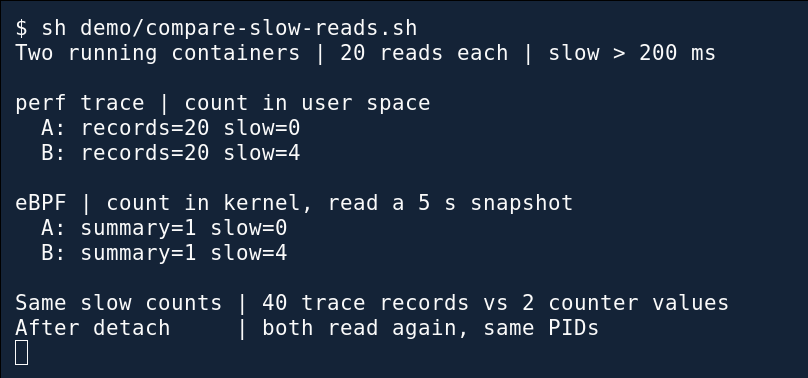
\includegraphics[width=\linewidth]{images/demo-slow-reads-terminal.png}
    \end{column}
    \begin{column}{0.30\textwidth}
      \begin{block}{Cùng kết quả}
        A có \textbf{0}, B có \textbf{4} lượt đọc chậm.
      \end{block}
      \begin{block}{Dữ liệu nhận được}
        \texttt{perf trace}: \textbf{40} bản ghi.\\
        eBPF: \textbf{2} giá trị tổng.
      \end{block}
    \end{column}
  \end{columns}
  \vspace{0.22cm}
  \centering\textbf{Sau khi gỡ probe, cả hai tiến trình đọc tiếp với cùng PID.}
  \note{Ảnh từ terminal khi chạy demo thật. 40 là số bản ghi của các lượt đọc mẫu mà script perf xử lý. 2 là số giá trị tổng theo container ở lần đọc map đầu tiên. Phép đo không đếm các gói nội bộ hay đo CPU.}
\end{frame}

\begin{frame}[fragile]{Phép đo eBPF trên kernel đang chạy}
  \small
  Hai tracepoint tại đầu và cuối \texttt{read()} cung cấp mốc thời gian cho phép đo.
  \vspace{0.20cm}
  \begin{columns}[T,onlytextwidth]
    \begin{column}{0.43\textwidth}
      \begin{block}{Lọc và đếm bên ngoài kernel}
        \begin{lstlisting}
perf trace -a -G "$path_a" -e read
\end{lstlisting}
        Script đọc thời lượng từ từng dòng trace rồi đếm các lượt trên 200 ms.
      \end{block}
    \end{column}
    \begin{column}{0.52\textwidth}
      \begin{block}{Lọc và đếm trong kernel}
        \lstinputlisting[firstline=17,lastline=19]{demo/slow-reads.bt}
        Probe cộng vào bộ đếm của container. Sau 5 giây, công cụ giám sát đọc số tổng.
      \end{block}
    \end{column}
  \end{columns}
  \vspace{0.30cm}
  \begin{center}
    \textbf{Phép đo có thể bắt đầu và kết thúc trong khi máy chủ\\
      tiếp tục phục vụ các container.}
  \end{center}
  \note{Trích mã thực thi. Probe được kernel kiểm tra khi nạp và cần hook cùng quyền phù hợp. Bản đầy đủ lưu thời điểm bắt đầu theo TID và xóa trạng thái khi lượt đọc kết thúc.}
\end{frame}

% Chapter 02: content from chaptersnew, diagrams from the existing template.
\section{Chương 2: Kiến trúc eBPF}
\ChapterDivider{Chương 2}{Kiến trúc eBPF}{Chương trình chạy ở đâu và các thành phần phối hợp thế nào?}

\begin{frame}{eBPF nằm ở đâu trong Linux?}
  \begin{center}
    \begin{tikzpicture}[font=\small]
      \draw[draw=BKTemplate, fill=BKTemplate!4, rounded corners=3pt] (0,3.45) rectangle (14.1,5.3);
      \node[anchor=west, font=\small\bfseries, text=BKTemplate] at (0.2,5.05) {User Space};
      \node[ebpfuser, text width=4.4cm, minimum height=0.9cm] (app) at (3.5,4.3)
        {Ứng dụng thông thường\\Yêu cầu dịch vụ kernel};
      \node[ebpfuser, text width=5.0cm, minimum height=0.9cm] (tool) at (10.7,4.3)
        {\textbf{bpftrace / libbpf}\\Nạp chương trình, thu thập kết quả};
      \draw[draw=gray!65!black, fill=gray!4, rounded corners=3pt] (0,0.8) rectangle (14.1,2.95);
      \node[anchor=west, font=\small\bfseries] at (0.2,2.7) {Kernel Space};
      \node[ebpfkernel, text width=6.0cm, minimum height=1.1cm] (services) at (3.8,1.7)
        {\textbf{Quản lý hệ thống}\\Scheduler \quad File System\\Memory Management \quad Network Stack};
      \node[ebpfprogram, text width=4.7cm, minimum height=1.1cm] (prog) at (10.7,1.7)
        {\textbf{Chương trình eBPF}\\Thực thi tại hook được hỗ trợ};
      \draw[arr] (app.south) -- node[right, font=\footnotesize, fill=white, inner sep=2pt] {System calls} (services.north);
      \draw[arr, dashed] (tool.south) -- node[right, font=\footnotesize, fill=white, inner sep=2pt] {BPF API} (prog.north);
      \node[key, minimum width=14.1cm, minimum height=0.7cm] (hw) at (7.05,-0.05)
        {\textbf{Hardware}\hspace{1cm} CPU\hspace{1cm}RAM\hspace{1cm}Thiết bị I/O};
      \draw[arr] (7.05,0.8) -- (hw.north);
    \end{tikzpicture}
  \end{center}
  \note{Công cụ như bpftrace hoặc ứng dụng dùng libbpf hoạt động ở User Space. Các mũi tên biểu thị vai trò, không phải toàn bộ chuỗi nạp chương trình. Chương trình eBPF thực thi trong ngữ cảnh phù hợp với program type và hook. Nguồn: \url{https://docs.kernel.org/bpf/libbpf/libbpf_overview.html}; \url{https://docs.kernel.org/bpf/verifier.html}.}
\end{frame}

\begin{frame}{Kiến trúc eBPF: chuẩn bị và thực thi}
  \begin{center}
    \begin{tikzpicture}[font=\small,
      prep/.style={arr, draw=BKTemplate, dashed},
      run/.style={arr, draw=green!45!black}]
      \node[anchor=west, text=BKTemplate, font=\small\bfseries] at (-0.9,0.95) {A. Chuẩn bị chương trình};
      \node[ebpfuser, text width=2.1cm, minimum height=1.0cm] (loader) at (0.3,-0.2) {Userspace\\Loader};
      \node[ebpfkernel, text width=2.2cm, minimum height=1.0cm] (verifier) at (4.0,-0.2) {Verifier\\\footnotesize Kiểm tra khi nạp};
      \node[ebpfprogram, text width=2.4cm, minimum height=1.0cm] (loaded) at (7.9,-0.2) {eBPF Program\\\footnotesize Được chấp nhận nạp};
      \node[ebpfkernel, text width=2.1cm, minimum height=1.0cm] (attached) at (11.8,-0.2) {Hook\\\footnotesize Tương thích};
      \draw[prep] (loader) -- node[above, font=\footnotesize] {Load} (verifier);
      \draw[prep] (verifier) -- (loaded);
      \draw[prep] (loaded) -- node[above, font=\footnotesize] {Attach} (attached);
      \node[key, text width=12.7cm, font=\footnotesize, align=left, fill=white, minimum height=0.7cm] at (6.0,-1.53)
        {\textbf{JIT (tùy chọn):} Dịch bytecode thành mã máy khi được hỗ trợ và bật. JIT không phải hook.};
      \node[anchor=west, text=green!40!black, font=\small\bfseries] at (-0.9,-2.5) {B. Khi sự kiện xảy ra};
      \node[ebpfkernel, text width=1.75cm, minimum height=1.1cm] (event) at (0.1,-3.4) {Kernel\\Event};
      \node[ebpfkernel, text width=1.45cm, minimum height=1.1cm] (hook) at (2.85,-3.4) {Hook};
      \node[ebpfprogram, text width=2.05cm, minimum height=1.1cm] (prog) at (5.7,-3.4) {eBPF\\Program};
      \node[ebpfmap, text width=1.85cm, minimum height=1.1cm, font=\footnotesize] (data) at (9.0,-3.4) {Map /\\event output};
      \node[ebpfuser, text width=2.05cm, minimum height=1.1cm] (user) at (12.3,-3.4) {Userspace\\Application};
      \draw[run] (event) -- (hook);
      \draw[run] (hook) -- (prog);
      \draw[run] (prog) -- (data);
      \draw[run] (data) -- (user);
      \node[font=\footnotesize, align=left, text width=14.0cm, anchor=west] at (-0.9,-4.52)
        {\textbf{Map:} Program dùng helper/cơ chế phù hợp. User Space đọc qua \texttt{bpf()} hoặc libbpf.};
      \node[font=\footnotesize, text=gray!75!black, anchor=west] at (-0.9,-5.13)
        {Verifier kiểm tra khi nạp, không kiểm tra lại mỗi lần có sự kiện.};
    \end{tikzpicture}
  \end{center}
  \note{Luồng A nét đứt mô tả load, verify và attach. Luồng B nét liền mô tả sự kiện và dữ liệu. Map và cơ chế gửi sự kiện là các lựa chọn truyền kết quả, không phải mọi chương trình đều dùng cả hai. Với map, helper/cơ chế phù hợp dùng phía kernel, còn bpf()/libbpf dùng từ User Space. JIT là tùy chọn, không phải điều kiện bắt buộc để nạp. Nguồn: \url{https://docs.kernel.org/bpf/libbpf/libbpf_overview.html}; \url{https://docs.kernel.org/bpf/maps.html}; \url{https://docs.kernel.org/admin-guide/sysctl/net.html}.}
\end{frame}

\begin{frame}{Bốn thành phần cốt lõi của eBPF}
  \small
  \begin{columns}[T,onlytextwidth]
    \begin{column}{0.48\textwidth}
      \begin{block}{eBPF Program}
        Logic xử lý, chạy trong ngữ cảnh do program type quy định.
      \end{block}
      \begin{block}{Hook}
        Điểm gắn chương trình: tracepoint, kprobe, XDP.\\[0.1cm]
        Phải tương thích với program type.
      \end{block}
    \end{column}
    \begin{column}{0.48\textwidth}
      \begin{block}{eBPF Map}
        Lưu trạng thái, bộ đếm và chia sẻ dữ liệu với User Space.
      \end{block}
      \begin{block}{Verifier}
        Kiểm tra luồng điều khiển, bộ nhớ và thao tác được phép khi nạp.
      \end{block}
    \end{column}
  \end{columns}
  \vspace{0.20cm}
  \textcolor{BKTemplate}{Verifier không bảo đảm đúng logic. Chương trình vẫn có chi phí xử lý.}
  \note{Mỗi program type có ngữ cảnh và các thao tác được phép riêng. Không phải chương trình nào cũng gắn vào mọi hook. Map có nhiều loại và API khác nhau. Verifier kiểm tra các điều kiện an toàn trước khi chấp nhận nạp, không chứng minh logic ứng dụng hoàn toàn đúng. Nguồn: \url{https://docs.kernel.org/bpf/verifier.html}; \url{https://docs.kernel.org/bpf/maps.html}; \url{https://docs.kernel.org/bpf/libbpf/program_types.html}.}
\end{frame}

\begin{frame}{Luồng xử lý một sự kiện}
  \noindent{\small Ví dụ: một tiến trình thực hiện system call.}\par
  \vspace{0.10cm}
  \begin{center}
    \begin{tikzpicture}[font=\small]
      \node[ebpfkernel, text width=3.4cm, minimum height=0.85cm] (call) at (0,0) {System call};
      \node[ebpfkernel, text width=3.4cm, minimum height=0.85cm] (hook) at (4.7,0) {Tracepoint / Hook};
      \node[ebpfprogram, text width=3.4cm, minimum height=0.85cm] (prog) at (9.4,0) {eBPF Program};
      \node[ebpfprogram, text width=3.4cm, minimum height=1.1cm] (process) at (9.4,-1.7)
        {Lọc, lấy thông tin,\\cập nhật bộ đếm};
      \node[ebpfmap, text width=3.4cm, minimum height=1.1cm] (data) at (4.7,-1.7)
        {Map hoặc cơ chế\\gửi sự kiện};
      \node[ebpfuser, text width=3.4cm, minimum height=1.1cm] (user) at (0,-1.7) {User Space};
      \draw[arr] (call) -- (hook);
      \draw[arr] (hook) -- (prog);
      \draw[arr] (prog) -- (process);
      \draw[arr] (process) -- (data);
      \draw[arr] (data) -- (user);
    \end{tikzpicture}
  \end{center}
  \vspace{0.08cm}
  \cue{1}{Chương trình được \textbf{nạp và gắn trước} khi sự kiện xảy ra.}
  \cue{2}{Hook chỉ kích hoạt các chương trình được gắn phù hợp.}
  \cue{3}{Dữ liệu thu thập phụ thuộc program type, hook và logic xử lý.}
  \note{Sơ đồ khái quát cho sự kiện tại thời điểm system call đi vào kernel, không xác nhận lời gọi đã thành công. Các mũi tên chỉ mô tả luồng xử lý và dữ liệu. Những thao tác và dữ liệu được phép phụ thuộc program type, hook và kernel.}
\end{frame}

% Chapter 03 -- Content from chaptersnew, diagrams styled as chapters/.
\section{Chương 3: Phát triển và công cụ}
\ChapterDivider{Chương 3}{Phát triển và công cụ}{Từ mã nguồn đến quan sát được sự kiện thật}

\begin{frame}{Quy trình phát triển chương trình eBPF}
  \noindent{\small Ví dụ với C, Clang/LLVM và libbpf.}\par
  \begin{center}
    \begin{tikzpicture}
      \node[ebpfuser, text width=3.7cm, minimum height=1.9cm, align=left] (write) at (0,0)
        {\begin{minipage}[t][1.5cm][t]{3.7cm}\raggedright
         \textbf{1. Write}\\[0.13cm]
         Viết chương trình eBPF bằng C.
         \end{minipage}};
      \node[ebpfuser, text width=3.7cm, minimum height=1.9cm, align=left] (compile) at (4.7,0)
        {\begin{minipage}[t][1.5cm][t]{3.7cm}\raggedright
         \textbf{2. Compile}\\[0.13cm]
         Clang/LLVM tạo object chứa bytecode.
         \end{minipage}};
      \node[ebpfkernel, text width=3.7cm, minimum height=1.9cm, align=left] (load) at (9.4,0)
        {\begin{minipage}[t][1.5cm][t]{3.7cm}\raggedright
         \textbf{3. Load \& Verify}\\[0.13cm]
         Loader yêu cầu nạp, Verifier kiểm tra.
         \end{minipage}};
      \node[ebpfkernel, text width=3.7cm, minimum height=1.9cm, align=left] (attach) at (9.4,-2.5)
        {\begin{minipage}[t][1.5cm][t]{3.7cm}\raggedright
         \textbf{4. Attach}\\[0.13cm]
         Gắn program vào hook tương thích.
         \end{minipage}};
      \node[ebpfprogram, text width=3.7cm, minimum height=1.9cm, align=left] (execute) at (4.7,-2.5)
        {\begin{minipage}[t][1.5cm][t]{3.7cm}\raggedright
         \textbf{5. Execute}\\[0.13cm]
         Sự kiện phù hợp kích hoạt program.
         \end{minipage}};
      \node[ebpfmap, text width=3.7cm, minimum height=1.9cm, align=left] (collect) at (0,-2.5)
        {\begin{minipage}[t][1.5cm][t]{3.7cm}\raggedright
         \textbf{6. Collect}\\[0.13cm]
         User Space đọc map hoặc nhận sự kiện.
         \end{minipage}};
      \draw[arr] (write) -- (compile);
      \draw[arr] (compile) -- (load);
      \draw[arr] (load) -- (attach);
      \draw[arr] (attach) -- (execute);
      \draw[arr] (execute) -- (collect);
    \end{tikzpicture}
  \end{center}
  {\small \textbf{Load và Attach là hai bước riêng.} JIT là tùy chọn. Công cụ cấp cao có thể tự xử lý nhiều bước.}
  \note{Đây là quy trình ví dụ với C/libbpf. Loader yêu cầu kernel nạp chương trình; Verifier kiểm tra trong bước nạp. JIT có thể dịch bytecode sang mã máy khi được hỗ trợ và bật. bpftrace có thể quản lý nhiều bước thay người dùng. Nguồn: \url{https://docs.kernel.org/bpf/libbpf/libbpf_overview.html}; \url{https://docs.kernel.org/admin-guide/sysctl/net.html}.}
\end{frame}

\begin{frame}{Công cụ phát triển và sử dụng eBPF}
  \begin{center}
    \begin{tikzpicture}
      \node[ebpfuser, text width=6.0cm, minimum height=1.95cm, align=left] at (0,0)
        {\begin{minipage}[t][1.55cm][t]{6.0cm}\raggedright
         \textbf{bpftrace}\\[0.13cm]
         Tracing nhanh bằng cú pháp ngắn, phù hợp minh họa sự kiện.
         \end{minipage}};
      \node[ebpfuser, text width=6.0cm, minimum height=1.95cm, align=left] at (7.3,0)
        {\begin{minipage}[t][1.55cm][t]{6.0cm}\raggedright
         \textbf{bpftool}\\[0.13cm]
         Kiểm tra tính năng BPF của kernel. Quản lý program, map và link.
         \end{minipage}};
      \node[ebpfuser, text width=6.0cm, minimum height=1.95cm, align=left] at (0,-2.5)
        {\begin{minipage}[t][1.55cm][t]{6.0cm}\raggedright
         \textbf{libbpf}\\[0.13cm]
         Thư viện C hỗ trợ nạp, gắn và quản lý chương trình eBPF.
         \end{minipage}};
      \node[ebpfuser, text width=6.0cm, minimum height=1.95cm, align=left] at (7.3,-2.5)
        {\begin{minipage}[t][1.55cm][t]{6.0cm}\raggedright
         \textbf{BCC}\\[0.13cm]
         Thư viện và công cụ tracing để phân tích hành vi, hiệu năng hệ thống.
         \end{minipage}};
    \end{tikzpicture}
  \end{center}
  {\small \textbf{Thực hành:} Dùng \texttt{bpftool} kiểm tra môi trường và \texttt{bpftrace} theo dõi system calls, đếm sự kiện. Chưa cần tự viết loader bằng C.}
  \note{Vai trò và lựa chọn cho phần thực hành theo nội dung chaptersnew. Nguồn: \url{https://bpftrace.org/about}; \url{https://github.com/libbpf/bpftool/blob/main/docs/bpftool.rst}; \url{https://docs.kernel.org/bpf/libbpf/libbpf_overview.html}; \url{https://github.com/iovisor/bcc}.}
\end{frame}

\begin{frame}{Ví dụ: Theo dõi lời gọi \texttt{openat()}}
  \small
  Đếm lời gọi \texttt{openat()} yêu cầu mở tệp hoặc thư mục, thống kê theo \texttt{comm}.
  \begin{center}
    \begin{tikzpicture}
      \node[ebpfuser, text width=2.05cm, minimum height=2.4cm] (app) at (0,0)
        {\textbf{Application}\\[0.15cm]Gọi\\\texttt{openat()}};
      \node[ebpfkernel, text width=2.7cm, minimum height=2.4cm] (hook) at (3.0,0)
        {\textbf{Tracepoint}\\[0.15cm]\footnotesize\texttt{syscalls:}\\\texttt{sys\_enter\_openat}};
      \node[ebpfprogram, text width=2.15cm, minimum height=2.4cm] (prog) at (6.1,0)
        {\textbf{eBPF Program}\\[0.15cm]Lấy \texttt{comm}, cập nhật bộ đếm};
      \node[ebpfmap, text width=2.0cm, minimum height=2.4cm] (map) at (9.0,0)
        {\textbf{eBPF Map}\\[0.15cm]Số lần gọi theo\\\texttt{comm}};
      \node[ebpfuser, text width=2.15cm, minimum height=2.4cm] (user) at (11.9,0)
        {\textbf{bpftrace}\\[0.15cm]Đọc map, hiển thị thống kê};
      \draw[arr] (app) -- (hook);
      \draw[arr] (hook) -- (prog);
      \draw[arr] (prog) -- (map);
      \draw[arr] (map) -- (user);
    \end{tikzpicture}
  \end{center}
  \cue{1}{\texttt{comm} là tên tác vụ/tiến trình, không phải PID. Nhiều tiến trình có thể trùng tên.}
  \cue{2}{Sự kiện tại \textsl{entry} ghi nhận yêu cầu, chưa xác nhận mở tệp thành công.}
  \note{Sơ đồ minh họa cách bpftrace thu thập và hiển thị bộ đếm theo comm, không phải mã hay kết quả demo đã chạy. Tên tác vụ do kernel cung cấp có thể thay đổi và bị giới hạn độ dài. Tracepoint sys_enter_openat xảy ra khi bắt đầu lời gọi. Nguồn: \url{https://bpftrace.org/docs/release_024/language}; \url{https://man7.org/linux/man-pages/man5/proc_pid_comm.5.html}; \url{https://man7.org/linux/man-pages/man2/openat.2.html}.}
\end{frame}

% Chapter 04: chỉ bổ sung kết quả từ môi trường demo thật.
\section{Chương 4: Thực hành}
\ChapterDivider{Chương 4}{Thực hành}{Kiểm tra môi trường, theo dõi system call và thống kê sự kiện}

% Giữ khung nét đứt và màu của bộ slide hiện có.
\newcommand{\DemoPlaceholder}[5][Mục tiêu]{%
  \begin{frame}{#2}
    \begin{block}{#1}
      \small #3
    \end{block}
    \vspace{0.12cm}
    \begin{center}
      \begin{tikzpicture}
        \node[rectangle, draw=BKTemplate!60, dashed, line width=0.8pt,
          text width=12.5cm, minimum height=#5,
          text=gray, align=center, font=\small, inner sep=0.25cm] {#4};
      \end{tikzpicture}
    \end{center}
    {\small\textcolor{BKTemplate}{\textbf{TODO: Demo content will be added later}}}
  \end{frame}%
}

\DemoPlaceholder[Ba nội dung thực hành]{Thực hành: từ sơ đồ đến sự kiện thật}
  {\cue{1}{\textbf{Kiểm tra môi trường}: kernel, công cụ và quyền sử dụng BPF.}
   \cue{2}{\textbf{Theo dõi \texttt{execve()}}: tiến trình và chương trình được yêu cầu thực thi.}
   \cue{3}{\textbf{Đếm \texttt{openat()}}: nhóm theo \texttt{comm} bằng map, đọc ở User Space.}}
  {Sơ đồ tổng quan hoặc ảnh môi trường demo\\[0.20cm]
   \footnotesize Bổ sung sau khi chạy thử trên máy của nhóm.}
  {2.7cm}

\DemoPlaceholder{Demo 1: Kiểm tra môi trường eBPF}
  {Xác nhận phiên bản Linux kernel, công cụ, quyền chạy và các tính năng eBPF được máy demo hỗ trợ.}
  {Terminal hoặc ảnh chụp kết quả kiểm tra\\[0.20cm]
   \footnotesize Sử dụng kết quả từ chính môi trường demo của nhóm.}
  {3.15cm}

\DemoPlaceholder{Demo 2: Theo dõi system call \texttt{execve()}}
  {Ghi nhận PID và đường dẫn chương trình được yêu cầu thực thi khi tiến trình gọi \texttt{execve()}.}
  {Câu lệnh, terminal và kết quả tracing\\[0.20cm]
   \footnotesize Sự kiện tại entry ghi nhận yêu cầu, chưa xác nhận lời gọi thành công.}
  {3.15cm}

\DemoPlaceholder{Demo 3: Thống kê \texttt{openat()} bằng map}
  {Đếm \texttt{openat()} theo \texttt{comm} (tên tác vụ/tiến trình), lưu trong map và xem thống kê từ User Space.}
  {Câu lệnh, bảng đếm và phân tích đầu ra\\[0.20cm]
   \footnotesize \texttt{comm} không phải PID và có thể trùng giữa các tiến trình.\\[0.12cm]
   Số liệu chỉ được bổ sung sau khi thực hiện demo thật.}
  {3.15cm}


\end{document}
